\documentclass[11pt,a4paper]{article}
\usepackage[margin=1in]{geometry}
\usepackage[T1]{fontenc}
\usepackage[utf8]{inputenc}
\usepackage{lmodern}
\usepackage{hyperref}
\usepackage{enumitem}
\usepackage{xurl}
\usepackage{tikz}
\usepackage{float}
\usetikzlibrary{arrows.meta, positioning, shapes.geometric}
\hypersetup{colorlinks=true,linkcolor=blue,urlcolor=blue}
\newcommand{\codepath}[1]{\path{#1}}
\tikzset{
  box/.style={rectangle,draw,rounded corners,align=center,inner sep=3pt,minimum width=44mm},
  decision/.style={diamond,draw,aspect=2.2,align=center,inner sep=2pt},
  line/.style={-Latex}
}

\title{Phase-2 Deliverable: Spike Simulator Adapter}
\author{SIT Engine Documentation}
\date{\today}

\begin{document}
\maketitle

\section{Technical Description}
Spike adapter converts Spike execution traces into ingest-contract state and residency intervals using marker-aware parsing and deterministic timeline normalization.

\section{Implementation Fulfillment}
Implemented in \codepath{Phase-2/adapters/spike_adapter.py}; invoked by \codepath{Phase-2/riscvbench.py} for \texttt{--target spike}; validated by fixture/invariant/determinism tests.

\section{Design \& Architecture}
\subsection*{Function Attributes}
\begin{itemize}[leftmargin=*]
  \item \texttt{SpikePlatformAdapter.\_iter\_events()}: Inputs=spike trace lines; Outputs=ordered (core,mnemonic,pc,time) events; Side effects=extracts markers and instruction stream; Failure modes=unexpected log formats, parse drop.
  \item \texttt{SpikePlatformAdapter.\_collect\_core\_timeline()}: Inputs=parsed events + config; Outputs=per-core state/residency timelines; Side effects=applies marker-first residency logic; Failure modes=timeline gaps, marker mismatch.
  \item \texttt{build\_state\_intervals()}: Inputs=core timelines; Outputs=state intervals DataFrame; Side effects=classifies active/stall/idle segments; Failure modes=empty or malformed intervals.
  \item \texttt{build\_residency\_intervals()}: Inputs=core timelines; Outputs=residency intervals DataFrame; Side effects=emits resident windows; Failure modes=missing residency windows.
  \item \texttt{export\_baseline\_csvs()}: Inputs=normalized DataFrames + outdir; Outputs=state/residency CSV paths; Side effects=writes contract artifacts; Failure modes=file write failure, validation error.
\end{itemize}
\subsection*{Function Execution Details}
\begin{enumerate}[leftmargin=*]
  \item \texttt{SpikePlatformAdapter.\_iter\_events()}
  \begin{itemize}[leftmargin=*]
    \item Input attributes: spike trace lines.
    \item Processing flow: extracts markers and instruction stream.
    \item Output attributes: ordered (core,mnemonic,pc,time) events.
    \item Failure behavior: unexpected log formats, parse drop.
  \end{itemize}
  \item \texttt{SpikePlatformAdapter.\_collect\_core\_timeline()}
  \begin{itemize}[leftmargin=*]
    \item Input attributes: parsed events + config.
    \item Processing flow: applies marker-first residency logic.
    \item Output attributes: per-core state/residency timelines.
    \item Failure behavior: timeline gaps, marker mismatch.
  \end{itemize}
  \item \texttt{build\_state\_intervals()}
  \begin{itemize}[leftmargin=*]
    \item Input attributes: core timelines.
    \item Processing flow: classifies active/stall/idle segments.
    \item Output attributes: state intervals DataFrame.
    \item Failure behavior: empty or malformed intervals.
  \end{itemize}
  \item \texttt{build\_residency\_intervals()}
  \begin{itemize}[leftmargin=*]
    \item Input attributes: core timelines.
    \item Processing flow: emits resident windows.
    \item Output attributes: residency intervals DataFrame.
    \item Failure behavior: missing residency windows.
  \end{itemize}
  \item \texttt{export\_baseline\_csvs()}
  \begin{itemize}[leftmargin=*]
    \item Input attributes: normalized DataFrames + outdir.
    \item Processing flow: writes contract artifacts.
    \item Output attributes: state/residency CSV paths.
    \item Failure behavior: file write failure, validation error.
  \end{itemize}
\end{enumerate}


\subsection*{Diagram A: End-to-End Design Flow}
\begin{figure}[H]
\centering
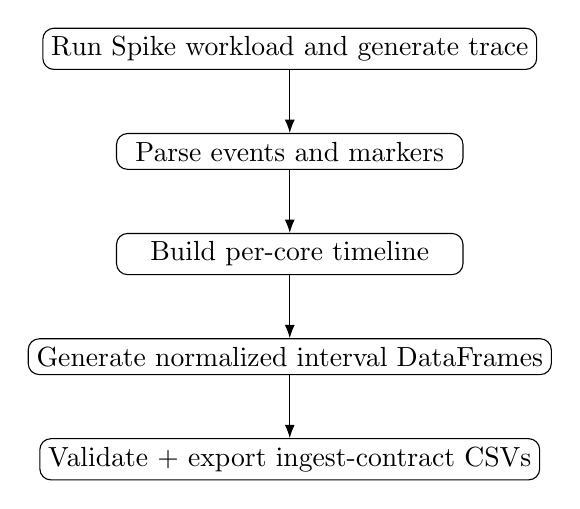
\begin{tikzpicture}[node distance=8mm and 12mm]
\node[box] (a) {Run Spike workload and generate trace};
\node[box, below=of a] (b) {Parse events and markers};
\node[box, below=of b] (c) {Build per-core timeline};
\node[box, below=of c] (d) {Generate normalized interval DataFrames};
\node[box, below=of d] (e) {Validate + export ingest-contract CSVs};
\draw[line] (a) -- (b);
\draw[line] (b) -- (c);
\draw[line] (c) -- (d);
\draw[line] (d) -- (e);
\end{tikzpicture}
\caption{Deliverable 02: End-to-End Design Flow}
\end{figure}

\subsection*{Diagram B: Function Interaction and Attribute Flow}
\begin{figure}[H]
\centering
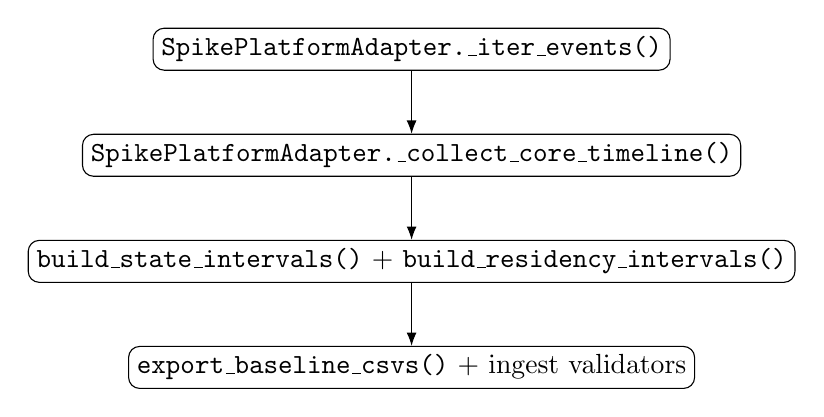
\begin{tikzpicture}[node distance=8mm and 12mm]
\node[box] (fa) {\texttt{SpikePlatformAdapter.\_iter\_events()}};
\node[box, below=of fa] (fb) {\texttt{SpikePlatformAdapter.\_collect\_core\_timeline()}};
\node[box, below=of fb] (fc) {\texttt{build\_state\_intervals()} + \texttt{build\_residency\_intervals()}};
\node[box, below=of fc] (fd) {\texttt{export\_baseline\_csvs()} + ingest validators};
\draw[line] (fa) -- (fb);
\draw[line] (fb) -- (fc);
\draw[line] (fc) -- (fd);
\end{tikzpicture}
\caption{Deliverable 02: Function Interaction and Attribute Flow}
\end{figure}

\end{document}
